
% 1. Lets start by creating a report document! use \documentclass{report} 
\documentclass{report} 
% 2. Uncomment the following preamble packages to load options for figures
% Preamble
\usepackage{graphicx} % for figures
\usepackage{subcaption} % for subplots 
\usepackage[labelsep=space,tableposition=top]{caption}
\renewcommand{\figurename}{Fig.} 
\usepackage{cleveref}
% 3. Create a title and author using \title and \author{names}. Begin document, 
%and insert the title using \maketitle
\title{King's College, Cambridge}
\author{Krishna Kumar \thanks{grad.computing@kings.cam.ac.uk}}

% 4. Uncomment to insert list of figures: \listoffigures

\graphicspath{{figs/}}

\begin{document}
\maketitle
\listoffigures
\clearpage

\section{King's College, Cambridge}


King's College is a constituent college of the University of Cambridge, 
England. The college's full name is ``The King's College of our Lady and Saint 
Nicholas in Cambridge'', but it is usually referred to simply as ``King's''
within the University.

The college was founded in 1441 by King Henry VI, soon after its sister college 
in Eton. However, the King's plans for the college were disrupted by the civil 
war and resultant scarcity of funds, and his eventual deposition. Little 
progress was made on the project until in 1508 King Henry VII began to take an 
interest in the college, most likely as a political move to legitimise his new 
position. The building of the college's chapel, begun in 1446, was finally 
finished in 1544 during the reign of King Henry VIII.


% 5. To create a figure use the float \begin{figure} \end{figure}. Inserting a 
%picture requires graphicx package. 
% 6. To include the figure use \includegraphics[options]{name}. name usually 
%specifies the location of the figure. Recommend using a directory to hold all 
%the figures. Options include the size / width. 
% 7. Uncomment [htbp!] the options specify location of the figure. [h-here, 
%t-top, b-bottom, p-para and !-override] try using one at a time and see the 
%location of figures. 
% LaTeX usually tries to place the figures closer to where it has been 
%referenced!

\begin{figure}[b] %[tbhp!] 
\centering    %remove comment
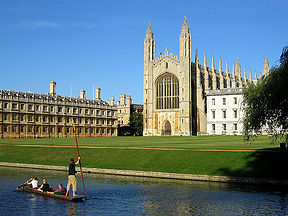
\includegraphics[width=0.7\textwidth]{figs/Kings.png}
\caption[King's College Cambridge]{``The King's College of our Lady and Saint 
Nicholas in Cambridge'', but it is usually referred to simply as ``King's'' 
within the University of Cambridge, England.}
\label{fig:Kings}
\end{figure}

% 8. Referencing the figure is done using \cref{unique_label}. Label of the 
%figures should be unique. 

King's College Chapel (see~\cref{fig:Kings}) is regarded as one of the 
greatest examples of late Gothic English architecture. It has the world's 
largest fan-vault, and the chapel's stained-glass windows and wooden chancel 
screen are considered some of the finest from their era. The building is seen 
as emblematic of Cambridge. The chapel's choir, composed of male students at 
King's and choristers from the nearby King's College School, is one of the most 
accomplished and renowned in the world. Every year on Christmas Eve the 
Festival of Nine Lessons and Carols (a service created by a Dean of King's 
especially for the college) is broadcast from the chapel to millions of 
listeners worldwide.


\section*{Subplots}

I can cite Wall-E (see~\cref{fig:WallE}) and Minions in despicable me 
(\cref{fig:Minnion}).~\Cref{fig:animations} lets me cite the whole figure.

% 9. A subplot can be created inside the figure environment using 
%\begin{subfigure} and \includegraphics{name} for each subfigure. Please use  
%subcaption package instead of subfig. Also align the subfigures vertically 
%instead of horizontally.

\begin{figure}
  \centering
  \begin{subfigure}[b]{0.3\textwidth}
    
\includegraphics[width=\textwidth]{TomandJerry.png}
    \caption{Tom and Jerry}
    \label{fig:TomJerry}   
  \end{subfigure}          \\   
  \begin{subfigure}[b]{0.3\textwidth}
    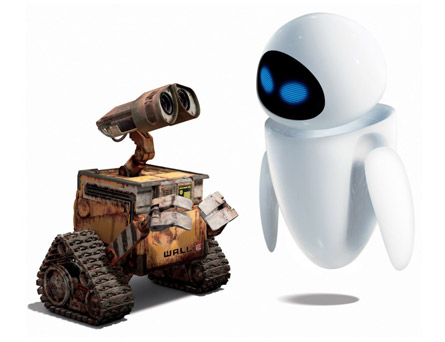
\includegraphics[width=\textwidth]{WallE}
    \caption{Wall-E}
    \label{fig:WallE}
  \end{subfigure}            \\ 
  \begin{subfigure}[b]{0.3\textwidth}
    
\includegraphics[width=\textwidth]{minion}
    \caption{A Minion}
    \label{fig:Minnion}
  \end{subfigure}
  \caption{Best Animations}
  \label{fig:animations}
\end{figure}

\end{document}